%% March 2018
%%%%%%%%%%%%%%%%%%%%%%%%%%%%%%%%%%%%%%%%%%%%%%%%%%%%%%%%%%%%%%%%%%%%%%%%%%%%
% AGUJournalTemplate.tex: this template file is for articles formatted with LaTeX
%
% This file includes commands and instructions
% given in the order necessary to produce a final output that will
% satisfy AGU requirements, including customized APA reference formatting.
%
% You may copy this file and give it your
% article name, and enter your text.
%
%
% Step 1: Set the \documentclass
%
% There are two options for article format:
%
% PLEASE USE THE DRAFT OPTION TO SUBMIT YOUR PAPERS.
% The draft option produces double spaced output.
%

%% To submit your paper:
\documentclass[]{agujournal2018}
\usepackage{apacite}
\usepackage{url} %this package should fix any errors with URLs in refs.
%%%%%%%
% As of 2018 we recommend use of the TrackChanges package to mark revisions.
% The trackchanges package adds five new LaTeX commands:
%
%  \note[editor]{The note}
%  \annote[editor]{Text to annotate}{The note}
%  \add[editor]{Text to add}
%  \remove[editor]{Text to remove}
%  \change[editor]{Text to remove}{Text to add}
%
% complete documentation is here: http://trackchanges.sourceforge.net/
%%%%%%%


%% Enter journal name below.
%% Choose from this list of Journals:
%
% JGR: Atmospheres
% JGR: Biogeosciences
% JGR: Earth Surface
% JGR: Oceans
% JGR: Planets
% JGR: Solid Earth
% JGR: Space Physics
% Global Biogeochemical Cycles
% Geophysical Research Letters
% Paleoceanography and Paleoclimatology
% Radio Science
% Reviews of Geophysics
% Tectonics
% Space Weather
% Water Resources Research
% Geochemistry, Geophysics, Geosystems
% Journal of Advances in Modeling Earth Systems (JAMES)
% Earth's Future
% Earth and Space Science
% Geohealth
%
% ie, \journalname{Water Resources Research}

\journalname{Water Resources Research}

\usepackage{soulutf8}

\begin{document}

%% ------------------------------------------------------------------------ %%
%  Title
%
% (A title should be specific, informative, and brief. Use
% abbreviations only if they are defined in the abstract. Titles that
% start with general keywords then specific terms are optimized in
% searches)
%
%% ------------------------------------------------------------------------ %%

% Example: \title{This is a test title}

\title{AquaSat: a dataset to enable remote sensing of water quality for inland
waters}

%% ------------------------------------------------------------------------ %%
%
%  AUTHORS AND AFFILIATIONS
%
%% ------------------------------------------------------------------------ %%

% Authors are individuals who have significantly contributed to the
% research and preparation of the article. Group authors are allowed, if
% each author in the group is separately identified in an appendix.)

% List authors by first name or initial followed by last name and
% separated by commas. Use \affil{} to number affiliations, and
% \thanks{} for author notes.
% Additional author notes should be indicated with \thanks{} (for
% example, for current addresses).

% Example: \authors{A. B. Author\affil{1}\thanks{Current address, Antartica}, B. C. Author\affil{2,3}, and D. E.
% Author\affil{3,4}\thanks{Also funded by Monsanto.}}

\authors{
Matthew R.V. Ross
\affil{1}
Simon N. Topp
\affil{2}
Alison P. Appling
\affil{3}
Xiao Yang
\affil{2}
Catherine Kuhn
\affil{4}
David Butman
\affil{4}
Marc Simard
\affil{5}
Tamlin Pavelsky
\affil{2}
}


% \affiliation{1}{First Affiliation}
% \affiliation{2}{Second Affiliation}
% \affiliation{3}{Third Affiliation}
% \affiliation{4}{Fourth Affiliation}

\affiliation{1}{Department of Ecosystem Science and Sustainability, Colorado State
University,}
\affiliation{2}{Department of Geological Sciences, University of North Carolina}
\affiliation{3}{United States Geological Survey}
\affiliation{4}{School of Environmental and Forest Sciences, University of Washington}
\affiliation{5}{NASA Jet Propulsion Laboratory}
%(repeat as many times as is necessary)

%% Corresponding Author:
% Corresponding author mailing address and e-mail address:

% (include name and email addresses of the corresponding author.  More
% than one corresponding author is allowed in this LaTeX file and for
% publication; but only one corresponding author is allowed in our
% editorial system.)

% Example: \correspondingauthor{First and Last Name}{email@address.edu}
\correspondingauthor{Matthew R.V. Ross}{matt.ross@colostate.edu}

%% Keypoints, final entry on title page.

%  List up to three key points (at least one is required)
%  Key Points summarize the main points and conclusions of the article
%  Each must be 100 characters or less with no special characters or punctuation

% Example:
% \begin{keypoints}
% \item	List up to three key points (at least one is required)
% \item	Key Points summarize the main points and conclusions of the article
% \item	Each must be 100 characters or less with no special characters or punctuation
% \end{keypoints}

\begin{keypoints}
\item AquaSat contains \textgreater{}550,000 paired observations of water
quality and Landsat reflectance, the largest such matchup dataset
\item Matchups capture diverse waterbodies across the USA for 1984-2018; we
see clear water quality/reflectance relationships
\item AquaSat and open source code developed here will enable better
development of models for remote sensing of water quality
\end{keypoints}

%% ------------------------------------------------------------------------ %%
%
%  ABSTRACT
%
% A good abstract will begin with a short description of the problem
% being addressed, briefly describe the new data or analyses, then
% briefly states the main conclusion(s) and how they are supported and
% uncertainties.
%% ------------------------------------------------------------------------ %%

%% \begin{abstract} starts the second page

\begin{abstract}
Satellite predictions of inland water quality have the potential to
vastly expand our ability to observe and monitor the dynamics of large
water bodies. For almost 50 years, we have been able to remotely sense
key water quality constituents like Total Suspended Sediment (TSS),
Dissolved Organic Carbon (DOC), Chlorophyll a, and Secchi Disk Depth
(SDD). Nonetheless, remote sensing of water quality is poorly integrated
into inland water sciences, in part due to a lack of publicly available
training data and a perception that remote estimates are unreliable.
Remote sensing models of water quality can be improved by training and
validation on larger datasets of coincident field and satellite
observations, here called matchups. To facilitate model development and
deeper integration of remote sensing into inland water science, we have
built AquaSat, the largest such matchup dataset ever assembled. AquaSat
contains more than 550,000 matchups, covering 1984-2018, of ground-based
TSS, DOC, Chlorophyll a, and SDD measurements paired with spectral
reflectance from Landsat 5, 7, and 8 collected within +/-1 day of each
other. To build AquaSat, we developed open source tools in R and Python
and applied them to existing public datasets covering the contiguous
United States, including the Water Quality Portal, LAGOS, and the
Landsat archive. In addition to publishing the dataset, we are also
publishing our full code architecture to facilitate expanding and
improving AquaSat. We anticipate that this work will help make remote
sensing of inland water accessible to more hydrologists, ecologists, and
limnologists while facilitating novel data-driven approaches to
monitoring and understanding critical water resources at large
spatiotemporal scales.\\
\end{abstract}

\section{Introduction}

Production and effective dissemination of water quality data is a vital
first step towards understanding natural and anthropogenic drivers of
aquatic ecosystem change \citep{Srebotnjak2012}. Collecting such
valuable data has historically been expensive and time-consuming, and it
has often proved difficult to maintain analysis-ready and open datasets.
In many developed nations, however, data access and interoperability
have been actively addressed over the last 10-20 years, leading to the
publication and maintenance of large open-access data repositories of
water quality measurements
\citep{Lack2000,Ballantine2014,Read2017,Soranno2017}, but over a limited
number of water bodies. Furthermore, access to robust historic water
quality sampling data remains limited to a few economically developed
countries \citep{Sheffield2018}.

With satellite remote sensing, we can augment \emph{in-situ} sampling
efforts and provide water quality information in places with little or
no data. Since the beginning of the Landsat missions, limnologists,
oceanographers, and hydrologists have been interested in developing
universal algorithms for extracting water quality information from
remotely sensed images
\citep{Clarke1970,Klemas1973,Maul1975,Ritchie1976,Holyer1978}. From
these early efforts, fifty years of work have used spectral information
to predict water quality parameters like total suspended solids (TSS),
chlorophyll a (here abbreviated as Chl\_a), colored dissolved organic
matter (CDOM), and Secchi disk depth (SDD). However, progress towards
universal algorithms and unified approaches has been slow
\citep{Bukata2013,Blondeau-Patissier2014,Palmer2015,Gholizadeh2016}
especially at the global scale. Further, most papers published to date
have focused on developing predictive methods as opposed to using
predictions to interrogate processes that control water quality dynamics
(Topp et al., \emph{in review}).

This slow progress contrasts sharply with ocean remote sensing, which
benefits from robust, open and big datasets geared towards pairing both
\emph{in-situ} and radiometric observations with satellite data,
enabling rapid development of more universally effective algorithms and
approaches \citep{Blondeau-Patissier2014,Bukata2013}. Ocean remote
sensing also benefits from dedicated satellites designed specifically
for ocean applications such as remote retrieval of Chl\_a, but the
spatial resolution of these sensors is too coarse to resolve most inland
waterbodies. As a result, inland water remote sensing has been limited
to satellites built for terrestrial remote sensing \citep{Palmer2015}.
Methods development for inland waters is further challenged by the
greater optical complexity of inland waters, where spectral signatures
reflect a mixture of inorganic suspended sediment, organic suspended
sediment, algae, dissolved organic matter, and other constituents. We
think some of these inherent challenges in inland water quality remote
sensing can be met at a broad scale because with a centralized, public
remote sensing dataset paired with \emph{in-situ} measurements of water
quality \citep{Palmer2015}.

In this data paper, we present AquaSat, a merged dataset of
\emph{in-situ} water quality measurements paired with same-day or
\(\pm\) 1-day satellite reflectance (which we call ``matchups''). This
is the largest such matchup dataset ever assembled for inland waters. To
create AquaSat, we use the Landsat archive from 1984-2018, available in
its entirety on the Google Earth Engine platform \citep{Gorelick2017},
in combination with data from the Water Quality Portal (WQP, Read et
al., 2017) and the LAke multi-scaled GeOSpatial and temporal database
covering the northeastern United States (LAGOS-NE, Soranno et al.,
2017). The WQP data we used covers all of the USA. Joining these
datasets provides us with an unprecedented resource to model, predict,
and understand the long-term and large-scale dynamics of variation in
TSS, SDD, Chl\_a, and dissolved organic carbon (DOC). We also outline
and share our approach, code, and intermediate data for bringing the
WQP, LAGOS-NE, and Landsat datasets together.

\section{Methods}

\subsection{Parameter description}

We focused on five common water quality parameters often targeted for
remote sensing of water quality: TSS, DOC and CDOM, Chlorophyll a and
Chl\_a. These four parameters capture key ecological and physical
factors that control water quality, and capabilities to remotely sense
each of them have been demonstrated (Topp et al., \emph{in review}).

TSS is a measure of the concentration of solids, both organic and
inorganic, in a water column, measured in mg/L. Waters with higher TSS
generally scatter more sunlight at all visible and near-infrared
wavelengths \citep{Ritchie1976}. Knowing TSS concentrations can provide
insight into subsurface light conditions \citep{Julian2008}, erosion
conditions \citep{Syvitski2011}, and the hydrologic status of
waterbodies, where high TSS generally means sediment supply coupled with
higher flow velocities \citep{Williams1989,Pavelsky2009}.

DOC, measured in mg/L, is the broad description for the concentration of
organic carbon dissolved in water, and can provide insight into light
conditions \citep{Vahatalo2005}, heterotrophic energy availability
\citep{Robbins2017}, and terrestrial organic matter processing
\citep{Williamson2008}. While DOC does not inherently alter the optical
properties of water, its colored portion, CDOM, does affect optics and
is often correlated with DOC concentration
\citep{Bricaud1981,Griffin2011} (Bricaud et al., 1981; Griffin et al.,
2011). This correlation between CDOM and DOC can break down in places
with low DOC concentrations \citep{Griffin2018}, or in areas with high
photobleaching of DOC, which alters the DOC/CDOM fractionation
\citep{Spencer2009,Cory2015}.

Chlorophyll a is a photosynthetically active pigment contained in all
phytoplankton. Chlorophyll a can be used to detect algae blooms
\citep{Kutser2004}, estimate primary productivity \citep{Antoine1996},
and understand algae dynamics \citep{Richardson1996}.

Finally, we gathered data on Secchi disk depth (typically measured in
meters), a long-standing method for estimating water clarity
\citep{Secchi1864,Lee2018}. SDD is a simple measurement that integrates
the optical properties of all water constituents and can provide
information on the trophic status of waterbodies \citep{Carlson1977} or
the algal status of a waterbody \citep{Lorenzen1980}.

\subsection{Data Sources}

Combining \emph{in-situ} data with the Landsat surface reflectance
archive first requires a large repository of water quality samples in
order to increase the probability of spatiotemporally co-located
satellite and field samples. For this paper, we focused on the two
largest databases of water quality in the United States: the WQP and
LAGOS-NE. These datasets contrast in important ways: one has more data,
emphasizing data quantity (WQP) and the other has more quality
assurances (LAGOS-NE). Using both ensures sampling the largest possible
number of waterbodies, while retaining a harmonized, analysis-ready
subset of the data.

\subsubsection{Water Quality Portal}

The WQP, with mostly data from the USA, is the largest observation
dataset of water quality in the world. The WQP houses more than 290
million observations at 2.7 million sites dating back more than a
century \citep{Read2017}. The WQP continuously gathers water quality
information from more than 450 organizations including academic,
government, NGO, tribal, and state datasets \citep{Read2017}. These data
streams are then distributed in a standardized format, facilitating
analysis across collection methods. While there is no entity that
harmonizes the data across providers \citep{Read2017}, subsets of the
data have been used in many publications analyzing water quality change
in the USA \citep{Booth2011,Sprague2009,Oelsner2017}. As with many large
datasets, the diversity of data sources and variation in meta-data
quality pose significant challenges to directly using the WQP as an
analysis-ready dataset \citep{Sprague2017}. Instead, end-users must
carefully harmonize data across sampling methods, analytic approaches,
and measurement units. The nature of harmonizing such large, distributed
data generates a necessary trade-off between a deep, time-consuming
exploration of data interoperability and a shallower, less
time-consuming, but potentially more error-prone data quality check.

\subsubsection{LAGOS-NE}

The LAGOS project (which generated the dataset LAGOS-NE) was, in part,
designed to address some of the data harmonization issues inherent to
the WQP, with the explicit goal of building a publicly available
high-quality dataset for continental-scale lake analyses
\citep{Soranno2015,Soranno2017}. In addition to pairing \emph{in-situ}
lake data with physical lake characteristics and local geologic setting,
LAGOS researchers harmonized key water quality measurements across the
87 water quality datasets that they gathered
\citep{Soranno2015,Soranno2017}. Because LAGOS researchers combined data
from many different sources, they chose to identify all data for a
single lake with the lake centroid. If two different organizations were
measuring Secchi disk depth at the north and south end of a lake, the
LAGOS dataset would combine all of these measurements into a single time
series, located at the lake centroid. For same day observations, the
deepest observation would have been kept \citep{Soranno2015}. This
approach is different from that used by the WQP, which often includes
multiple sites and depths per water body and simultaneous observations.
In its current form, the LAGOS-NE dataset covers only lakes in the
Northeast and Midwest, two lake-rich regions of the USA. LAGOS-NE
(v1.087.1) provides a dataset of the highest quality for matching
\emph{in-situ} data to Landsat overpasses.

\subsubsection{Landsat}

For this project, we joined the \emph{in-situ} database (WQP and
LAGOS-NE) with the Landsat Tier 1 products. The Landsat program started
in July 1972, as the Earth Resources Observation Satellite with an
explicit mission to provide solutions for some of earth's pressing
issues associated with industry and environmental change
\citep{Loveland2012}. For this project we are only using the three most
recent Landsat mission datasets: Landsat 5 (Thematic Mapper, 1984-2012,
192745 available images), Landsat 7 (Enhanced Thematic Mapper +,
1999-present, 197564 images), and Landsat 8 (Operational Land Imager,
2013-present, 69030 images). The total number of usable images is
significantly lower because of cloud cover, which varies greatly by
region and season. Furthermore, on May 31, 2003, the Landsat 7 scan line
corrector failed, causing the Landsat 7 images after this date to have
striped data gaps \citep{Storey2005}. We included all Landsat 7 data
before and after this date, but did not fill gaps associated with the
scan line error. The orbit repeat period of all three satellites is
sixteen days, though at high latitudes overlapping images result in
shorter revisit times \citep{Loveland2012,Wulder2016}. In most of the
USA, a given location will be imaged at least once every sixteen days,
and during periods of mission overlap, images are available on average
at least every eight days.

Landsat 5 and 7 have onboard imagers that collect seven bands of imagery
centered on three visible wavelengths (blue, green, and red) and four
infrared wavelengths (near infrared, shortwave infrared 1, shortwave
infrared 2, and thermal band). Designed for continuity with previous
sensors, Landsat 8 has bands in the same spectral regions and improved
signal-to-noise ratios, with an additional ultra-blue band
\citep{Barsi2014}. Landsat 7 and 8 have panchromatic bands at 15m
resolution, while Landsat 5 does not. To keep matchup data in a standard
format across time, we chose to use bands that were available and had
the same spatial resolution in at least two of the Landsat missions (SI
Table 1).

Satellite image data needs to be atmospherically corrected to account
for differences between what the satellite can image from space, and the
actual reflectance on the surface of the earth. When properly applied,
atmospheric corrections can reduce the interference of absorbing and
scattering aerosols, sun glint, and other processes that contribute to
the signal observed at the satellite over waterbodies, which can mask
the optical information from the waterbody itself \citep{Gordon1997}.
There are many options tailored for atmospheric correction over inland
waters available for users on a scene-by-scene basis, For large-scale
analysis, the USGS developed a surface reflectance product available in
Google Earth Engine which uses a version of the 6SV radiative transfer
model called Landsat Ecosystem Disturbance Adaptive Processing System
(LEDAPS) for Landsat 5 and 7 \citep{Ju2012} and the Landsat 8 Surface
Reflectance Code (LaSRC) for Landsat 8 \citep{Doxani2018,Vermote2016}.
While these surface reflectance products were developed for terrestrial
remote sensing and not inland-water observations, recent work by
\citet{Kuhn2019} demonstrates LaSRC performs well (within 4\% difference
of field radiometry) in estimating surface reflectance over the Amazon
river. Also, the USGS product is the only standardized reflectance
product that is globally available at the spatial scale required for
inland water observation. Users may want to apply other atmospheric
corrections, so while we only publish here the surface reflectance data,
our code can be used to work with top-of-atmosphere reflectance as well.

\subsection{Data integration}

Building this dataset required a flexible code architecture with a
single workflow to download data from all three portals. Steps in the
workflow included segmenting the data downloads into manageable pieces,
conducting quality assurance checks, and joining data into the final
data files (Figure \ref{fig:fig1}). To avoid redundant data transfers
and computations, we constructed a data pipeline that allowed us to only
update each intermediate data product when needed -- i.e., when related
sections of code were altered or when we wanted to bring in new source
data. We implemented the pipeline using the R package remake
\citep{FitzJohn2018}, which uses text files to declare the relationships
among data and code files, then reruns only the code that must be rerun
to keep the data up to date. The remake R package follows in the
tradition of the make program for compiling computer software
\citep{Feldman1979}. Although this project uses three different tools
(R, Python, and Google Earth Engine), each tool is called directly from
R -version 3.5.1 \citep{RFoundationforStatisticalComputing2018}- and
RMarkdown files \citep{Allaire2018}, such that remake could be used to
keep track of recent changes to code and data regardless of the tool.
This data pipeline approach made our own analysis more efficient and
should also increase efficiency for future researchers who may want to
recreate the dataset themselves or modify our specific approach.

\begin{figure}[h]
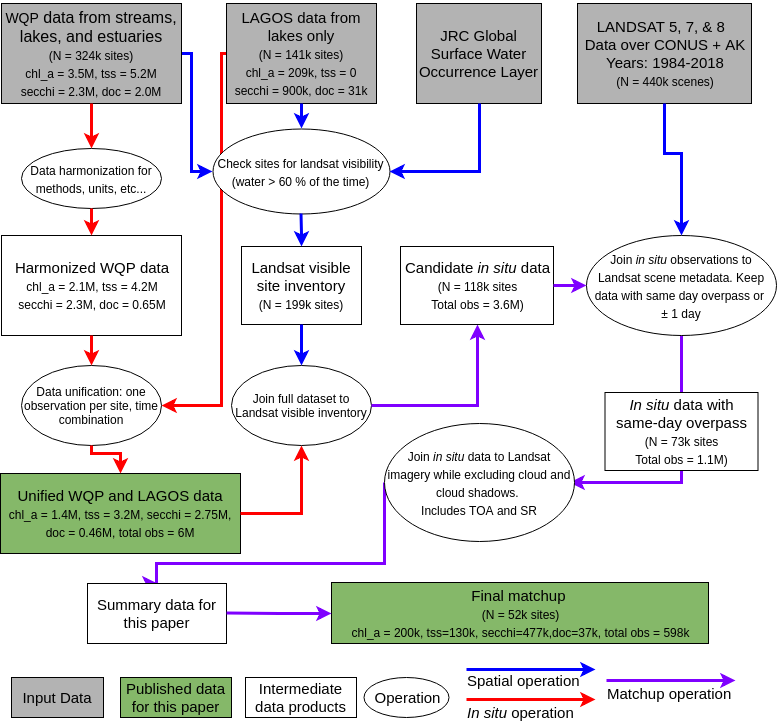
\includegraphics[width=1\linewidth,]{C:/Users/mrvr/Dropbox/UNC-PostDocAll/aquasat/4_report/src/AquaSat_WRR_Submission/Watersat_Drop_flow} \caption{Overview of data sources, steps taken to join data, and total observation counts}\label{fig:fig1}
\end{figure}

\subsubsection{Water quality data download and quality control}

We developed an automated method to retrieve our five water quality
parameters from the WQP and LAGOS sites. For the WQP we used the
dataRetrieval R package \citep{Hirsch2015}, which allows systematical
downloading of WQP data. The WQP contains hundreds of parameter types
(under the field ``characteristicName'' in the WQP), and we carefully
selected those that best represented our target parameters based on our
own expertise and previously published research using the same data
sources, see SI table 2 for more information
\citep{Butman2016,Stets2012}. For all selected parameters, we downloaded
data for all US states except Hawaii for four water body categories:
Lake, Reservoir, or Impoundment; Stream; Estuary; and Facility, where
facility can indicate wastewater treatment facilities, including lakes
and ponds. Finally, we restricted our queries to data sampled in water,
excluding sediment and benthic samples.

Working with the LAGOS-NE data required many fewer decisions to combine
parameters, since LAGOS researchers have already harmonized and combined
parameters into simple categories that reflect our general parameter
codes \citep{Soranno2015,Soranno2017}. LAGOS-NE includes measurements
of: DOC, Chl\_a, and SDD, but no data on TSS or CDOM. As with the WQP,
the dataset can be simply loaded using an R package called LAGOSNE
\citep{Soranno2017}.

Turning data from the WQP into an analysis-ready dataset similar to
LAGOS-NE requires a chain of decisions documented and justified in the
supplemental html file (SI 3). We have attempted to make these decisions
both clear and justifiable, with the end goal of producing a
high-quality dataset. Figure \ref{fig:fig1} presents these data quality
assurance procedures and shows how they reduce the number of
observations at each step. The following are the most important
decisions:

\begin{enumerate}
\def\labelenumi{\arabic{enumi}.}
\item
  All observations were verified to have analytical methods related to
  parameter name; when this was not the case, samples were dropped. For
  example, if an observation was supposed to report TSS, but the
  analytical method was listed as ``Nitrogen in Water,'' then that
  sample would be dropped. For TSS in particular, we assumed that the
  characteristicName ``Suspended Sediment Concentration'' reflected the
  same data as ``TSS'' despite some methodological differences in the
  data collection as documented by Gray and others (2000). However, we
  keep the original name so end-users of the data can filter based on
  method as they see fit.
\item
  We harmonized the data across exchangeable units such that TSS and DOC
  data are in mg/L, Chl\_a data is in \(mu\)g/L, and Secchi disk depth
  is in meters. We removed all observations with mismatched units
  (e.g.~SDD in mg/L).
\item
  Ideally all observations would include sample depth information for
  accurate pairing of surface water data with reflectance. However, only
  40\% of the harmonized water quality data has depth data. For
  observations that did have sample depth data, we removed all
  observations deeper than 100 meters (\textless{} 1\% of data), a depth
  where constituent concentration likely has little effect on radiation
  leaving the waterbody. For the samples with recorded depth, more than
  97\% of data were sampled within 20m of the surface of the waterbody,
  suggesting most samples are near surface.
\item
  We verified that both LAGOS-NE and WQP data have only one observation
  per site at a particular date and/or time. Some observations include
  date without timestamp; for our purposes we needed one observation per
  date if only date information was available and one per datetime if
  timestamps were recorded. Where the date, time, and observation value
  were the same for multiple observations, we converted duplicates to a
  single value. When the site and date or datetime were the same, but
  the parameter values were different, we averaged multiple observations
  to a single observation if the coefficient of variation (standard
  deviation/mean) was less than 10\% and removed observations with too
  many simultaneous observations (5 per date time combination) or too
  much variation with no metadata explaining the repeat observations.
\item
  TSS can be separated into subcategories by particle size (like sand,
  clay, silt fractions) or by particle type (organic or inorganic),
  because many TSS observations (\textgreater{} 400,000) included these
  fractioning datasets, we split them into two additional parameters of
  interest: fraction sand (p\_sand) and total inorganic sediment (tis).
  We kept fraction sand instead of clay and/or silt, because there was
  limited data on clay and silt fractions.
\item
  Finally, we elected to keep all non-negative values not excluded by
  the preceding steps, requiring users to conduct their own assessment
  of how well the data reflect their expert knowledge of the system and
  parameter.
\end{enumerate}

While other selection criteria could have been included to make all
observations fully consistent, we avoided choices that removed the
majority of the WQP data. For example, some analytical methods do not
measure the exact same thing, such as measuring chlorophyll a with a
fluorescence probe versus with high performance liquid chromatography.
If we elected to only keep perfectly exchangeable methods, a majority of
the data would be lost. To allow user-defined selections, we included
the methods attribute in an additional dataset. Some decisions that
resulted in retaining data included: not filtering data based on
sampling method, not including temperature data as a filter for DOC and
Chl\_a samples, and including data that had unlabeled sample fraction
metadata. While these decisions may preclude some types of analysis, our
free and open source code allows future researchers to choose different
data quality criteria and generate a strict or expanded dataset to match
user needs.

\section{Results}

The quality assurance steps yielded almost 600,000 \emph{in-situ}
samples that fell within \(\pm\) 1 day of a Landsat overpass. Matching
\emph{in-situ} data to Landsat overpasses limits the dataset to only
4-15\% of the total \emph{in-situ} observations (Figure \ref{fig:fig1}),
with the biggest reduction in TSS observations and the smallest in SDD.
This pattern stems from the fact that most TSS observations are made in
streams too small to be visible from Landsat, while SDD observations are
mostly in lakes, which are visible. Given this reduction, we elected to
remove CDOM from AquaSat because there were only 2761 \emph{in-situ}
CDOM results in the entire WQP, which would have resulted in less than
100 total matchups. The remaining data are well distributed across the
parts of the USA with many lakes and rivers, including the Upper
Midwest, Northeast, and Florida, with notable data concentrations near
the Chesapeake Bay and along the U.S. East Coast in major estuarine
environments (Figure \ref{fig:map}). The western United States has
notably less data available, which likely reflects lower concentrations
of lakes and rivers in these states, the lack of LAGOS-NE data for these
states, and, potentially, a bias in the completeness of the WQP towards
certain states.

\begin{figure}[h]
\includegraphics{AquaSat_WRR_Submission_files/figure-latex/map-1} \caption{Distribution of observations across the conterminous USA, binned by local region. The data is split by observation type, where total represents an overpass for any of the four primary parameters. Data for AK and HI not shown, though they are in the dataset.}\label{fig:map}
\end{figure}

Lake-heavy regions like Florida, Wisconsin, and Minnesota dominate the
dataset. They contribute 71\% of the data, mostly in the form of SDD
observations. Figure \ref{fig:map} shows that DOC is the rarest
observation in AquaSat, as it is in the \emph{in-situ} data (SI Fig 1).
Half of all data comes from sites with only one or two matchups and less
than 10\% of sites have 25 or more observations. Given this limitation,
reflectance-based water quality models borrowing information across many
sites may be the most efficient way to use the database. Still, there
are hundreds of sites for each parameter that have at least 50 matchups,
which presents exciting opportunities for site-specific remote sensing
research and possibly even assessments of water quality trends over
time.

The temporal distribution of available data in our matchup dataset
generally reflects the availability of data in WQP and LAGOS-NE and the
launch or retirement of Landsat missions (SI Fig 1). It also reflects
the original WQP data \citep{Read2017}, as there is increasing data
available in the \emph{in-situ} datasets from 1984 to 2012. The more
recent decline in data availability may reflect a lag between agencies
collecting data and submitting final datasets to the \emph{in-situ}
databases and decreased funding \citep{Myers2017} to monitoring
organizations.

\begin{figure}[h]
\includegraphics{AquaSat_WRR_Submission_files/figure-latex/captured-1} \caption{Data distributions for the *in-situ* data (gray) and the matchup data (red). Data quantiles are shown in the background as a color ramp from sage to blue, corresponding to the color scale in Figure 4. Quantiles were calculated for matchup data only.}\label{fig:captured}
\end{figure}

The data we captured in the matchup dataset reflects the distribution of
\emph{in-situ} data (Fig. \ref{fig:captured}). This is especially true
for Chl\_a and SDD, where the overpass distribution shapes are nearly
identical to the \emph{in-situ} distributions, just with fewer
observations. The matchup data misses the largest values for both DOC
and TSS, which occur almost entirely in small streams not visible to
Landsat. Across parameter values (depths or concentrations), the matchup
data spans several orders of magnitude and captures environmentally
meaningful variation in water quality. For each parameter, the data is
approximately log-normally distributed, with the majority of the data
occupying a relatively narrow range, within \textasciitilde{}1-2 orders
of magnitude of the median (Fig. \ref{fig:captured}).

Based on decades of previous research (Topp et al, in review WRR),
optically active constituents control absorption and scattering
properties of water bodies, which in turn impacts their reflectance.
While exploring these relationships at individual sites or regions is
beyond the scope of this paper, we interrogate the dataset to examine
how variation in each water quality constituent maps to variation in
reflectance in each spectral band. We divided AquaSat into the six
quantiles shown in figure \ref{fig:variation} for each water quality
parameter. Increasing concentrations of Chl\_a, DOC, and TSS or
increasing SDD control spectral variation, even when averaged across our
three waterbody types (Estuary, Stream, and Lake) and averaged for the
entire USA. Despite using such a heterogeneous dataset, figure
\ref{fig:variation} shows clear systematic variation in spectral
response for each parameter as concentration or SDD increases.

\begin{figure}[h]
\includegraphics{AquaSat_WRR_Submission_files/figure-latex/variation-1} \caption{Shows spectral response, scaled and dimensionless, for each data quantile for each Landsat band. For Chl\_a, DOC, and TSS, concentration increases moving from left to right for higher quantiles. For SDD, higher quantiles indicate increasing clarity or deeper SDD. The value range represented in each quantile are shown in figure 3.}\label{fig:variation}
\end{figure}

\section{Discussion}

To our knowledge, the AquaSat dataset is the largest matchup dataset
ever assembled for inland waters. Combining historical datasets of water
quality and satellite reflectance maximizes the information we can gain
from past data collections. Aquasat can inform our future approaches to
\emph{in-situ} water quality monitoring by, for example, targeting
sampling efforts near satellite overpass days. AquaSat, a dataset
essentially built on the overlapping of \emph{in-situ} water quality
monitoring and Landsat imaging schedules, captures a broad range of
variation in four major remotely observable water quality parameters
across thousands of waterbodies, and we anticipate it will unlock many
avenues for remote water quality work. The four parameters in AquaSat
(DOC, Chl\_a, SDD, TSS), within most of their range, have a significant
impact on the observed surface reflectance, showing promising results
for the value of this data to build predictive algorithms.

By publishing this data, we hope to contribute to the ongoing transition
in the field from primarily developing methods to one where those
methods are used to interrogate patterns in water quality and drivers of
water quality change (Topp et al, in review WRR). For example, with an
open, big dataset, method comparisons for predictive models can be
conducted, accelerating scientific discovery \citep{Bukata2013}. We
built this dataset to provide an easy way for non-experts in remote
sensing to begin using it into their research. Because the matchup data
covers the United States, this work could range from classic approaches
like building local water quality algorithms for detecting algae blooms
in a single lake to more regional and national work predicting TSS in
all the major rivers of the USA. We expect that as remote predictions of
inland water quality become more common, they can be used as a
complement to \emph{in-situ} datasets, vastly expanding our
understanding of water quality trends and current status across the USA
and world. We also anticipate that by enabling more work on remote
sensing of water quality, we can fill in some of the spatial biases in
water quality data that are inherent to the WQP and efforts like LAGOS.

We built AquaSat to move towards continental-and global-scale remote
sensing of water quality, but the dataset comes with caveats and
limitations. First and foremost, the WQP and LAGOS-NE have spatial
biases in terms of which water bodies were sampled, which agencies fully
report their data, and the completeness of records; these biases are
carried over into AquaSat. Second, our efforts to harmonize and unify
the data in the WQP were performed with the explicit goal of including
as much data as possible. Such inclusivity ensured a dataset that allows
future users the flexibility to set their own standards in line with the
requirements of their individual needs, but it comes with intentionally
limited quality. The LAGOS-NE dataset, which was more extensively
assured for quality, exemplifies a contrasting approach
\citep{Soranno2017,Soranno2015}. Lastly, for the remote sensing data, we
used published surface reflectance estimates developed primarily with
terrestrial remote sensing in mind, though recent work suggests these
approaches may be as effective as custom approaches \citep{Kuhn2019}.
For researchers who prefer their own atmospheric corrections, we also
provide code for pulling top-of-atmosphere reflectance, which has no
atmospheric correction applied.

Our approach of pairing public \emph{in-situ} and satellite data can be
expanded to any place with measurements of water quality. By publishing
our code, we encourage use of our approach or code in other countries,
moving towards truly global remote sensing of inland water quality.
Additionally, there is ample previous work showing that remote sensing
of water quality can be expanded to include constituents that are not
optically active but are correlated with TSS or DOC, like mercury
\citep{Fichot2016,Telmer2006} or phosphorus \citep{Kutser1995}. Finally,
this work can be adjusted to include other satellites with publicly
available optical imagery (like Sentinel 2) or even private satellites
with higher temporal and spatial resolution (like DigitalGlobe or
PLANET). Our hope is that the content and philosophy of AquaSat help to
accelerate progress in all of these areas.

\acknowledgments

The acknowledgments must list:

All code used to generate this dataset can be found at:
https://github.com/GlobalHydrologyLab/watersat. The data for this paper
come from the Landsat archive, LAGOSNE, and the Water Quality Portal.
All of this data is free to download and the paper details extensively
how we combined the datasets. Data generated by our work can be found at
CUAHSI, Zenodo, and NASA archives. Part of this work was conducted at
the Jzet Propulsion Laboratory, California Institute of Technology,
under a contract with the National Aeronautics and Space Administration.
SNT was funded by a NASA NESSF grant (\#80NSSC18K1398) for work on this
grant. APA was supported by the Integration Information Dissemination
Division of the U.S. Geological Survey. There are no conflicts of
interest to report.

\bibliography{aquasat.bib}


\end{document}
